% Three of Anya's houses, and the dots that say the row goes on — Geometry 20
% of the abacus (Hard).
%
% One house is a square with both diagonals and a right-angled roof — the ridge
% sits half a side above the eaves, so the slopes run at 45°. That pitch is part
% of the problem, not decoration: it puts each slope on the same line as the
% neighbour's diagonal, and those alignments are worth 8 more triangles of the
% 116 in the answer. Neighbours share a wall. Wordless, so it builds once for both languages. Line art only:
% every stroke is black and gets rewritten to currentColor.
\documentclass[tikz,dvisvgm,border=3pt]{standalone}
\begin{document}
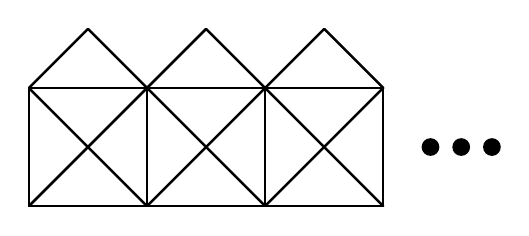
\begin{tikzpicture}[
  x=1.5cm, y=1.5cm,
  line join=round, line cap=round,
  edge/.style={line width=0.9pt},
]

\foreach \i in {0,1,2} {
  % the walls, with both diagonals
  \draw[edge] (\i,0) rectangle (\i+1,1);
  \draw[edge] (\i,0) -- (\i+1,1);
  \draw[edge] (\i,1) -- (\i+1,0);
  % the roof
  \draw[edge] (\i,1) -- (\i+0.5,1.5) -- (\i+1,1);
}

% …and so on
\foreach \i in {0,1,2} { \fill (3.4+0.26*\i,0.5) circle (0.075); }

\end{tikzpicture}
\end{document}
